\documentclass{article} % For LaTeX2e
\usepackage{iclr2022_conference,times}

% Optional math commands from https://github.com/goodfeli/dlbook_notation.
%%%%% NEW MATH DEFINITIONS %%%%%

\usepackage{amsmath,amsfonts,bm}

% Mark sections of captions for referring to divisions of figures
\newcommand{\figleft}{{\em (Left)}}
\newcommand{\figcenter}{{\em (Center)}}
\newcommand{\figright}{{\em (Right)}}
\newcommand{\figtop}{{\em (Top)}}
\newcommand{\figbottom}{{\em (Bottom)}}
\newcommand{\captiona}{{\em (a)}}
\newcommand{\captionb}{{\em (b)}}
\newcommand{\captionc}{{\em (c)}}
\newcommand{\captiond}{{\em (d)}}

% Highlight a newly defined term
\newcommand{\newterm}[1]{{\bf #1}}


% Figure reference, lower-case.
\def\figref#1{figure~\ref{#1}}
% Figure reference, capital. For start of sentence
\def\Figref#1{Figure~\ref{#1}}
\def\twofigref#1#2{figures \ref{#1} and \ref{#2}}
\def\quadfigref#1#2#3#4{figures \ref{#1}, \ref{#2}, \ref{#3} and \ref{#4}}
% Section reference, lower-case.
\def\secref#1{section~\ref{#1}}
% Section reference, capital.
\def\Secref#1{Section~\ref{#1}}
% Reference to two sections.
\def\twosecrefs#1#2{sections \ref{#1} and \ref{#2}}
% Reference to three sections.
\def\secrefs#1#2#3{sections \ref{#1}, \ref{#2} and \ref{#3}}
% Reference to an equation, lower-case.
\def\eqref#1{equation~\ref{#1}}
% Reference to an equation, upper case
\def\Eqref#1{Equation~\ref{#1}}
% A raw reference to an equation---avoid using if possible
\def\plaineqref#1{\ref{#1}}
% Reference to a chapter, lower-case.
\def\chapref#1{chapter~\ref{#1}}
% Reference to an equation, upper case.
\def\Chapref#1{Chapter~\ref{#1}}
% Reference to a range of chapters
\def\rangechapref#1#2{chapters\ref{#1}--\ref{#2}}
% Reference to an algorithm, lower-case.
\def\algref#1{algorithm~\ref{#1}}
% Reference to an algorithm, upper case.
\def\Algref#1{Algorithm~\ref{#1}}
\def\twoalgref#1#2{algorithms \ref{#1} and \ref{#2}}
\def\Twoalgref#1#2{Algorithms \ref{#1} and \ref{#2}}
% Reference to a part, lower case
\def\partref#1{part~\ref{#1}}
% Reference to a part, upper case
\def\Partref#1{Part~\ref{#1}}
\def\twopartref#1#2{parts \ref{#1} and \ref{#2}}

\def\ceil#1{\lceil #1 \rceil}
\def\floor#1{\lfloor #1 \rfloor}
\def\1{\bm{1}}
\newcommand{\train}{\mathcal{D}}
\newcommand{\valid}{\mathcal{D_{\mathrm{valid}}}}
\newcommand{\test}{\mathcal{D_{\mathrm{test}}}}

\def\eps{{\epsilon}}


% Random variables
\def\reta{{\textnormal{$\eta$}}}
\def\ra{{\textnormal{a}}}
\def\rb{{\textnormal{b}}}
\def\rc{{\textnormal{c}}}
\def\rd{{\textnormal{d}}}
\def\re{{\textnormal{e}}}
\def\rf{{\textnormal{f}}}
\def\rg{{\textnormal{g}}}
\def\rh{{\textnormal{h}}}
\def\ri{{\textnormal{i}}}
\def\rj{{\textnormal{j}}}
\def\rk{{\textnormal{k}}}
\def\rl{{\textnormal{l}}}
% rm is already a command, just don't name any random variables m
\def\rn{{\textnormal{n}}}
\def\ro{{\textnormal{o}}}
\def\rp{{\textnormal{p}}}
\def\rq{{\textnormal{q}}}
\def\rr{{\textnormal{r}}}
\def\rs{{\textnormal{s}}}
\def\rt{{\textnormal{t}}}
\def\ru{{\textnormal{u}}}
\def\rv{{\textnormal{v}}}
\def\rw{{\textnormal{w}}}
\def\rx{{\textnormal{x}}}
\def\ry{{\textnormal{y}}}
\def\rz{{\textnormal{z}}}

% Random vectors
\def\rvepsilon{{\mathbf{\epsilon}}}
\def\rvtheta{{\mathbf{\theta}}}
\def\rva{{\mathbf{a}}}
\def\rvb{{\mathbf{b}}}
\def\rvc{{\mathbf{c}}}
\def\rvd{{\mathbf{d}}}
\def\rve{{\mathbf{e}}}
\def\rvf{{\mathbf{f}}}
\def\rvg{{\mathbf{g}}}
\def\rvh{{\mathbf{h}}}
\def\rvu{{\mathbf{i}}}
\def\rvj{{\mathbf{j}}}
\def\rvk{{\mathbf{k}}}
\def\rvl{{\mathbf{l}}}
\def\rvm{{\mathbf{m}}}
\def\rvn{{\mathbf{n}}}
\def\rvo{{\mathbf{o}}}
\def\rvp{{\mathbf{p}}}
\def\rvq{{\mathbf{q}}}
\def\rvr{{\mathbf{r}}}
\def\rvs{{\mathbf{s}}}
\def\rvt{{\mathbf{t}}}
\def\rvu{{\mathbf{u}}}
\def\rvv{{\mathbf{v}}}
\def\rvw{{\mathbf{w}}}
\def\rvx{{\mathbf{x}}}
\def\rvy{{\mathbf{y}}}
\def\rvz{{\mathbf{z}}}

% Elements of random vectors
\def\erva{{\textnormal{a}}}
\def\ervb{{\textnormal{b}}}
\def\ervc{{\textnormal{c}}}
\def\ervd{{\textnormal{d}}}
\def\erve{{\textnormal{e}}}
\def\ervf{{\textnormal{f}}}
\def\ervg{{\textnormal{g}}}
\def\ervh{{\textnormal{h}}}
\def\ervi{{\textnormal{i}}}
\def\ervj{{\textnormal{j}}}
\def\ervk{{\textnormal{k}}}
\def\ervl{{\textnormal{l}}}
\def\ervm{{\textnormal{m}}}
\def\ervn{{\textnormal{n}}}
\def\ervo{{\textnormal{o}}}
\def\ervp{{\textnormal{p}}}
\def\ervq{{\textnormal{q}}}
\def\ervr{{\textnormal{r}}}
\def\ervs{{\textnormal{s}}}
\def\ervt{{\textnormal{t}}}
\def\ervu{{\textnormal{u}}}
\def\ervv{{\textnormal{v}}}
\def\ervw{{\textnormal{w}}}
\def\ervx{{\textnormal{x}}}
\def\ervy{{\textnormal{y}}}
\def\ervz{{\textnormal{z}}}

% Random matrices
\def\rmA{{\mathbf{A}}}
\def\rmB{{\mathbf{B}}}
\def\rmC{{\mathbf{C}}}
\def\rmD{{\mathbf{D}}}
\def\rmE{{\mathbf{E}}}
\def\rmF{{\mathbf{F}}}
\def\rmG{{\mathbf{G}}}
\def\rmH{{\mathbf{H}}}
\def\rmI{{\mathbf{I}}}
\def\rmJ{{\mathbf{J}}}
\def\rmK{{\mathbf{K}}}
\def\rmL{{\mathbf{L}}}
\def\rmM{{\mathbf{M}}}
\def\rmN{{\mathbf{N}}}
\def\rmO{{\mathbf{O}}}
\def\rmP{{\mathbf{P}}}
\def\rmQ{{\mathbf{Q}}}
\def\rmR{{\mathbf{R}}}
\def\rmS{{\mathbf{S}}}
\def\rmT{{\mathbf{T}}}
\def\rmU{{\mathbf{U}}}
\def\rmV{{\mathbf{V}}}
\def\rmW{{\mathbf{W}}}
\def\rmX{{\mathbf{X}}}
\def\rmY{{\mathbf{Y}}}
\def\rmZ{{\mathbf{Z}}}

% Elements of random matrices
\def\ermA{{\textnormal{A}}}
\def\ermB{{\textnormal{B}}}
\def\ermC{{\textnormal{C}}}
\def\ermD{{\textnormal{D}}}
\def\ermE{{\textnormal{E}}}
\def\ermF{{\textnormal{F}}}
\def\ermG{{\textnormal{G}}}
\def\ermH{{\textnormal{H}}}
\def\ermI{{\textnormal{I}}}
\def\ermJ{{\textnormal{J}}}
\def\ermK{{\textnormal{K}}}
\def\ermL{{\textnormal{L}}}
\def\ermM{{\textnormal{M}}}
\def\ermN{{\textnormal{N}}}
\def\ermO{{\textnormal{O}}}
\def\ermP{{\textnormal{P}}}
\def\ermQ{{\textnormal{Q}}}
\def\ermR{{\textnormal{R}}}
\def\ermS{{\textnormal{S}}}
\def\ermT{{\textnormal{T}}}
\def\ermU{{\textnormal{U}}}
\def\ermV{{\textnormal{V}}}
\def\ermW{{\textnormal{W}}}
\def\ermX{{\textnormal{X}}}
\def\ermY{{\textnormal{Y}}}
\def\ermZ{{\textnormal{Z}}}

% Vectors
\def\vzero{{\bm{0}}}
\def\vone{{\bm{1}}}
\def\vmu{{\bm{\mu}}}
\def\vtheta{{\bm{\theta}}}
\def\va{{\bm{a}}}
\def\vb{{\bm{b}}}
\def\vc{{\bm{c}}}
\def\vd{{\bm{d}}}
\def\ve{{\bm{e}}}
\def\vf{{\bm{f}}}
\def\vg{{\bm{g}}}
\def\vh{{\bm{h}}}
\def\vi{{\bm{i}}}
\def\vj{{\bm{j}}}
\def\vk{{\bm{k}}}
\def\vl{{\bm{l}}}
\def\vm{{\bm{m}}}
\def\vn{{\bm{n}}}
\def\vo{{\bm{o}}}
\def\vp{{\bm{p}}}
\def\vq{{\bm{q}}}
\def\vr{{\bm{r}}}
\def\vs{{\bm{s}}}
\def\vt{{\bm{t}}}
\def\vu{{\bm{u}}}
\def\vv{{\bm{v}}}
\def\vw{{\bm{w}}}
\def\vx{{\bm{x}}}
\def\vy{{\bm{y}}}
\def\vz{{\bm{z}}}

% Elements of vectors
\def\evalpha{{\alpha}}
\def\evbeta{{\beta}}
\def\evepsilon{{\epsilon}}
\def\evlambda{{\lambda}}
\def\evomega{{\omega}}
\def\evmu{{\mu}}
\def\evpsi{{\psi}}
\def\evsigma{{\sigma}}
\def\evtheta{{\theta}}
\def\eva{{a}}
\def\evb{{b}}
\def\evc{{c}}
\def\evd{{d}}
\def\eve{{e}}
\def\evf{{f}}
\def\evg{{g}}
\def\evh{{h}}
\def\evi{{i}}
\def\evj{{j}}
\def\evk{{k}}
\def\evl{{l}}
\def\evm{{m}}
\def\evn{{n}}
\def\evo{{o}}
\def\evp{{p}}
\def\evq{{q}}
\def\evr{{r}}
\def\evs{{s}}
\def\evt{{t}}
\def\evu{{u}}
\def\evv{{v}}
\def\evw{{w}}
\def\evx{{x}}
\def\evy{{y}}
\def\evz{{z}}

% Matrix
\def\mA{{\bm{A}}}
\def\mB{{\bm{B}}}
\def\mC{{\bm{C}}}
\def\mD{{\bm{D}}}
\def\mE{{\bm{E}}}
\def\mF{{\bm{F}}}
\def\mG{{\bm{G}}}
\def\mH{{\bm{H}}}
\def\mI{{\bm{I}}}
\def\mJ{{\bm{J}}}
\def\mK{{\bm{K}}}
\def\mL{{\bm{L}}}
\def\mM{{\bm{M}}}
\def\mN{{\bm{N}}}
\def\mO{{\bm{O}}}
\def\mP{{\bm{P}}}
\def\mQ{{\bm{Q}}}
\def\mR{{\bm{R}}}
\def\mS{{\bm{S}}}
\def\mT{{\bm{T}}}
\def\mU{{\bm{U}}}
\def\mV{{\bm{V}}}
\def\mW{{\bm{W}}}
\def\mX{{\bm{X}}}
\def\mY{{\bm{Y}}}
\def\mZ{{\bm{Z}}}
\def\mBeta{{\bm{\beta}}}
\def\mPhi{{\bm{\Phi}}}
\def\mLambda{{\bm{\Lambda}}}
\def\mSigma{{\bm{\Sigma}}}

% Tensor
\DeclareMathAlphabet{\mathsfit}{\encodingdefault}{\sfdefault}{m}{sl}
\SetMathAlphabet{\mathsfit}{bold}{\encodingdefault}{\sfdefault}{bx}{n}
\newcommand{\tens}[1]{\bm{\mathsfit{#1}}}
\def\tA{{\tens{A}}}
\def\tB{{\tens{B}}}
\def\tC{{\tens{C}}}
\def\tD{{\tens{D}}}
\def\tE{{\tens{E}}}
\def\tF{{\tens{F}}}
\def\tG{{\tens{G}}}
\def\tH{{\tens{H}}}
\def\tI{{\tens{I}}}
\def\tJ{{\tens{J}}}
\def\tK{{\tens{K}}}
\def\tL{{\tens{L}}}
\def\tM{{\tens{M}}}
\def\tN{{\tens{N}}}
\def\tO{{\tens{O}}}
\def\tP{{\tens{P}}}
\def\tQ{{\tens{Q}}}
\def\tR{{\tens{R}}}
\def\tS{{\tens{S}}}
\def\tT{{\tens{T}}}
\def\tU{{\tens{U}}}
\def\tV{{\tens{V}}}
\def\tW{{\tens{W}}}
\def\tX{{\tens{X}}}
\def\tY{{\tens{Y}}}
\def\tZ{{\tens{Z}}}


% Graph
\def\gA{{\mathcal{A}}}
\def\gB{{\mathcal{B}}}
\def\gC{{\mathcal{C}}}
\def\gD{{\mathcal{D}}}
\def\gE{{\mathcal{E}}}
\def\gF{{\mathcal{F}}}
\def\gG{{\mathcal{G}}}
\def\gH{{\mathcal{H}}}
\def\gI{{\mathcal{I}}}
\def\gJ{{\mathcal{J}}}
\def\gK{{\mathcal{K}}}
\def\gL{{\mathcal{L}}}
\def\gM{{\mathcal{M}}}
\def\gN{{\mathcal{N}}}
\def\gO{{\mathcal{O}}}
\def\gP{{\mathcal{P}}}
\def\gQ{{\mathcal{Q}}}
\def\gR{{\mathcal{R}}}
\def\gS{{\mathcal{S}}}
\def\gT{{\mathcal{T}}}
\def\gU{{\mathcal{U}}}
\def\gV{{\mathcal{V}}}
\def\gW{{\mathcal{W}}}
\def\gX{{\mathcal{X}}}
\def\gY{{\mathcal{Y}}}
\def\gZ{{\mathcal{Z}}}

% Sets
\def\sA{{\mathbb{A}}}
\def\sB{{\mathbb{B}}}
\def\sC{{\mathbb{C}}}
\def\sD{{\mathbb{D}}}
% Don't use a set called E, because this would be the same as our symbol
% for expectation.
\def\sF{{\mathbb{F}}}
\def\sG{{\mathbb{G}}}
\def\sH{{\mathbb{H}}}
\def\sI{{\mathbb{I}}}
\def\sJ{{\mathbb{J}}}
\def\sK{{\mathbb{K}}}
\def\sL{{\mathbb{L}}}
\def\sM{{\mathbb{M}}}
\def\sN{{\mathbb{N}}}
\def\sO{{\mathbb{O}}}
\def\sP{{\mathbb{P}}}
\def\sQ{{\mathbb{Q}}}
\def\sR{{\mathbb{R}}}
\def\sS{{\mathbb{S}}}
\def\sT{{\mathbb{T}}}
\def\sU{{\mathbb{U}}}
\def\sV{{\mathbb{V}}}
\def\sW{{\mathbb{W}}}
\def\sX{{\mathbb{X}}}
\def\sY{{\mathbb{Y}}}
\def\sZ{{\mathbb{Z}}}

% Entries of a matrix
\def\emLambda{{\Lambda}}
\def\emA{{A}}
\def\emB{{B}}
\def\emC{{C}}
\def\emD{{D}}
\def\emE{{E}}
\def\emF{{F}}
\def\emG{{G}}
\def\emH{{H}}
\def\emI{{I}}
\def\emJ{{J}}
\def\emK{{K}}
\def\emL{{L}}
\def\emM{{M}}
\def\emN{{N}}
\def\emO{{O}}
\def\emP{{P}}
\def\emQ{{Q}}
\def\emR{{R}}
\def\emS{{S}}
\def\emT{{T}}
\def\emU{{U}}
\def\emV{{V}}
\def\emW{{W}}
\def\emX{{X}}
\def\emY{{Y}}
\def\emZ{{Z}}
\def\emSigma{{\Sigma}}

% entries of a tensor
% Same font as tensor, without \bm wrapper
\newcommand{\etens}[1]{\mathsfit{#1}}
\def\etLambda{{\etens{\Lambda}}}
\def\etA{{\etens{A}}}
\def\etB{{\etens{B}}}
\def\etC{{\etens{C}}}
\def\etD{{\etens{D}}}
\def\etE{{\etens{E}}}
\def\etF{{\etens{F}}}
\def\etG{{\etens{G}}}
\def\etH{{\etens{H}}}
\def\etI{{\etens{I}}}
\def\etJ{{\etens{J}}}
\def\etK{{\etens{K}}}
\def\etL{{\etens{L}}}
\def\etM{{\etens{M}}}
\def\etN{{\etens{N}}}
\def\etO{{\etens{O}}}
\def\etP{{\etens{P}}}
\def\etQ{{\etens{Q}}}
\def\etR{{\etens{R}}}
\def\etS{{\etens{S}}}
\def\etT{{\etens{T}}}
\def\etU{{\etens{U}}}
\def\etV{{\etens{V}}}
\def\etW{{\etens{W}}}
\def\etX{{\etens{X}}}
\def\etY{{\etens{Y}}}
\def\etZ{{\etens{Z}}}

% The true underlying data generating distribution
\newcommand{\pdata}{p_{\rm{data}}}
% The empirical distribution defined by the training set
\newcommand{\ptrain}{\hat{p}_{\rm{data}}}
\newcommand{\Ptrain}{\hat{P}_{\rm{data}}}
% The model distribution
\newcommand{\pmodel}{p_{\rm{model}}}
\newcommand{\Pmodel}{P_{\rm{model}}}
\newcommand{\ptildemodel}{\tilde{p}_{\rm{model}}}
% Stochastic autoencoder distributions
\newcommand{\pencode}{p_{\rm{encoder}}}
\newcommand{\pdecode}{p_{\rm{decoder}}}
\newcommand{\precons}{p_{\rm{reconstruct}}}

\newcommand{\laplace}{\mathrm{Laplace}} % Laplace distribution

\newcommand{\E}{\mathbb{E}}
\newcommand{\Ls}{\mathcal{L}}
\newcommand{\R}{\mathbb{R}}
\newcommand{\emp}{\tilde{p}}
\newcommand{\lr}{\alpha}
\newcommand{\reg}{\lambda}
\newcommand{\rect}{\mathrm{rectifier}}
\newcommand{\softmax}{\mathrm{softmax}}
\newcommand{\sigmoid}{\sigma}
\newcommand{\softplus}{\zeta}
\newcommand{\KL}{D_{\mathrm{KL}}}
\newcommand{\Var}{\mathrm{Var}}
\newcommand{\standarderror}{\mathrm{SE}}
\newcommand{\Cov}{\mathrm{Cov}}
% Wolfram Mathworld says $L^2$ is for function spaces and $\ell^2$ is for vectors
% But then they seem to use $L^2$ for vectors throughout the site, and so does
% wikipedia.
\newcommand{\normlzero}{L^0}
\newcommand{\normlone}{L^1}
\newcommand{\normltwo}{L^2}
\newcommand{\normlp}{L^p}
\newcommand{\normmax}{L^\infty}

\newcommand{\parents}{Pa} % See usage in notation.tex. Chosen to match Daphne's book.

\DeclareMathOperator*{\argmax}{arg\,max}
\DeclareMathOperator*{\argmin}{arg\,min}

\DeclareMathOperator{\sign}{sign}
\DeclareMathOperator{\Tr}{Tr}
\let\ab\allowbreak


\usepackage{hyperref}
\usepackage{url}
\usepackage{amssymb}
\usepackage{graphicx}


\title{Hybrid recurrent model for regime switching nonstationary time series}

\author{Etienne DAVID \\
Heuritech \\
Paris \\
\texttt{etienne.david@heuritech.com} \\
\And
Sylvain Le Corff \\
Samovar, T\'el\'ecom SudParis, d\'epartement CITI, TIPIC \\
Institut Polytechnique de Paris, Palaiseau \\
\texttt{sylvain.le$\_$corff@telecom-sudparis.eu} \\
\And 
Jean Bellot \\
Heuritech \\
Paris \\
\texttt{jean.bellot@heuritech.com} \\
}

% The \author macro works with any number of authors. There are two commands
% used to separate the names and addresses of multiple authors: \And and \AND.
%
% Using \And between authors leaves it to \LaTeX{} to determine where to break
% the lines. Using \AND forces a linebreak at that point. So, if \LaTeX{}
% puts 3 of 4 authors names on the first line, and the last on the second
% line, try using \AND instead of \And before the third author name.

\newcommand{\fix}{\marginpar{FIX}}
\newcommand{\new}{\marginpar{NEW}}

\newcommand{\ts}{y}
\newcommand{\fullts}{{\bf \ts}}
\newcommand{\tspred}{\hat{\ts}}
\newcommand{\stat}{f}
\newcommand{\statparam}{\theta_{stat}}
\newcommand{\fullstat}{{\bf \stat}}
\newcommand{\lag}{h}
\newcommand{\window}{w}
\newcommand{\tswindow}{{\bf \ts}}
\newcommand{\meants}{\Bar{\ts}}
\newcommand{\rnnwindow}{{\bf \rnn}}
\newcommand{\rnn}{z}
\newcommand{\err}{err}
\newcommand{\errwindow}{{\bf \err}}
\newcommand{\rnnmodel}{\textsc{rnn}}
\newcommand{\ws}{w}
\newcommand{\fullws}{{\bf \ws}}
\newcommand{\wswindow}{{\bf \ws}}
\newcommand{\concatinput}{x}
\newcommand{\fullconcatinput}{{ \bf \concatinput}}
\newcommand{\numberts}{10000}
\newcommand{\threshold}{\eta}
\newcommand{\predictor}{RNN_p}
\newcommand{\classifier}{RNN_c}
\newcommand{\rnnparam}{\theta}
\newcommand{\remainder}{r}
\newcommand{\hiddenregime}{U}


%\iclrfinalcopy % Uncomment for camera-ready version, but NOT for submission.
\begin{document}


\maketitle

\begin{abstract}
Developing models and algorithms to draw causal inference for time series is a long standing statistical problem. It is crucial for many applications, in particular for fashion or retail industries, to make optimal inventory decisions and avoid massive wastes. By tracking thousands of fashion trends on social media with state-of-the-art computer vision approaches, we propose a new model for fashion time series forecasting. Our contribution is  twofold. We first provide the first fashion dataset gathering \numberts\ weekly fashion time series. As influence dynamics are the key of emerging trend detection, we associate with each time series several external weak signals representing behaviors of influencers towards the trend. Secondly, to leverage such a complex and rich dataset, we propose a new hybrid forecasting model. Our approach combines per-time-series parametric models with seasonal components and a global recurrent neural network to include sporadic external signals. This hybrid model provides state-of-the-art results on the fashion dataset, and illustrates the benefit of the contribution of external weak signals.
\end{abstract}

\section{Introduction}

Multivariate time series forecasting is a widespread statistical problem with  many applications, see for instance \citep{sarkka2013bayesian, douc2014nonlinear, zucchini2017hidden} and the numerous references therein.
 %Due to the diversity of applications and use cases, a multitude of models have been proposed. 
 Parametric generative models allow to provide explainable predictions with statistical guarantees based on a precise modeling of the predictive distributions of new data based on a record of past observations. %The parameters of these models are usually estimated using a sequence of observations of the target time series. 
Calibrating these models, for instance using maximum likelihood inference, often requires a fair amount of tuning to design a time series-specific model to provide  accurate forecasts and sharp confidence intervals.  Depending on the use case, statistical properties of the signal and the available data, many families of models have been proposed for time series.  The exponential smoothing model \citep{RePEc:inm:oropre:v:9:y:1961:i:5:p:673-685} or the ARIMA with the Box-Jenkins approach \citep{box2015time} are for instance very popular parametric linear generative models.  Hidden Markov models (HMM) are also widespread and presuppose that available observations are defined using missing data, possibly lying in a high dimensional state space, describing the dynamical system. This hidden state is assumed to be a Markov chain such that at each time step the received observation is a random function of the corresponding latent data.  Although hidden states are modeled as a Markov chain (or a mixing process)  the observations arising therefrom present a highly complex statistical structure. %Introducing latent hidden states, they assume that the predictive distribution is not unique and constant in time but multiple and lead by the values of the hidden states changing during time. 
 In various applications where signals exhibit non-stationarities such as trends and seasonality, classical HMM are not adapted. However, \citep{touron2017modeling}  recently proposed seasonal HMM, assuming that transition probabilities between the states, as well as the emission distributions, are not constant in time but evolve in a periodic manner. Strong consistency results were established in \citep{touron2019consistency} and Expectation Maximization based numerical experiments were proposed.
Altough these works provide promising results, HMM are computationally expensive to train and are not yet well studied for seasonal  sequences with thousands of components.
 
 %However, for a large part of applications, parametric generative approaches show limitation to capture  complexity. Accurate candidates can be found with latent data models.  

%During the past decades, forecasting applications have taken a totally new proportion. 
In many fields, single or few time series have become thousands of sequences with complex statistical structures. In this new context, classical time series specific statistical models show limitations when dealing with numerous heterogeneous data. Recurrent neural networks and recent sequence to sequence deep learning architectures offer very appealing numerical alternatives thanks to their capability of leveraging any kind of heterogeneous multivariate data, see for instance \citep{ hochreiter1997long,vaswani2017attention, salinas2020deepar, li2019enhancing, lim2019temporal}. %In the past decades, with the impressive results of deep neural networks (DNN) in vision or language, some time series forecasting applications have been proposed. 
Significant improvements have been achieved with Reccurent Neural Network and its Long Short-Term Memory (LSTM) or Gated Recurrent Unit (GRU)  declinations \citep{8614252}. 
A good example is the DeepAR model \citep{salinas2020deepar}. Based on a LSTM architecture, it can predict accurate probability distributions of the future of a sequence. More recently, applications using the Transformer model have been proposed  \citep{li2019enhancing}. A direct concurrent of the DeepAR model can be found with the Temporal Fusion Transformers (TFT) approach \citep{lim2019temporal}.  Unfortunately, they suffer from two main weaknesses. Firstly, many of them are "black-boxes"  as the final forecast usually does not come with a statistical guarantee  although a few recent works focused on measuring uncertainty in recurrent neural networks, see  \cite{martin2020monte}. Secondly, without a fine prepossessing and well chosen hyper-parameters, these methods could lead to poor results and are often outperformed by traditional statistical parametric models, see \cite{makridakis2018m4}.

In this paper, we consider  new time series forecasting application referred to as {\em fashion trends prediction}. Based on a cutting-edge image recognition technology, we built the first fashion dataset containing \numberts\ sequences representing the apparition of fashion trends on social media per week from 01-01-2015 to 01-01-2019. Our fashion time series has very appealing properties: they have all the same length, same seasonality, no missing value and the absence of sparse time series even for niche trends. The originality of our dataset come from the fact that additional external weak signals can be introduced. With our fashion expertise, we detected several groups of fashion users with a high influence power. Analysing their specific behaviours on social medias, we add to each time series, 4 external weak signals representing the same fashion trends but on a sub-category of users. We call them weak signals because they are often alerts or events that are too sparse, or too incomplete to allow on their own an accurate estimation of their impact on the prediction of the target signal. With this totally new application, we aim at designing a model able to deal with our large fashion dataset, leverage our complex external weak signals and finally provide the most accurate forecasts.
 
Recurrent neural network are appealing to tackle our forecasting problem due to their capability of leveraging external data.  Recently, hybrid models combining DNN architectures with widespread statistical models to deal with seasonality and trends have been proposed, see for instance  \citep{zhang2003time,jianwei2019novel,bandara2020lstm}. The approach providing the most striking results was proposed in  \citep{smyl2020hybrid} in the context of the M4 forecasting competition \citep{makridakis2020m4}.  Given a large dataset, a per-time-series multiplicative exponential smoothing model is introduced to estimate simple but fundamental components for each time series and compute a first prediction. Then a global recurrent neural network is trained on the entire dataset to correct errors of the previous exponential smoothing models. %With this process, the hybrid approach succeeds at mixing strengths of both model families: robustness of the time series specific parametric models and the power of neural network at learn complex dynamics on large dataset. 
%However, the hybrid model has not been designed to deal with external signals even if it include a neural network.

Following this work, we present in this paper a new hyrbid recurrent model for time series forecasting with inclusion of external weak signals. %We design a more general hybrid framework including the original multiplicative model and a new additive one. 
Our approach enriches existing hybrid models by incorporating an unobserved regime switching feature to account for the need neural network based correction. In order to leverage external signals, we modify the hybrid framework to allow the regime shift and the  global error-corrector neural network to deal with external data. By adding our fashion external weak signals in our proposed framework, we show the real potential of the hybrid approach: a global neural network, able to leverage large amount of data, deal with any kind of external weak signals, learn context and finally correct weaknesses and errors of any parametric models.

The paper is organized as follow. Section~\ref{sec:hybrid} describes our hybrid framework which consists of a per-time-series parametric model and a recurrent neural network combining the target sequences with external weak signals. Then, we present our new fashion dataset in Section~\ref{sec:dataset}. Section~\ref{sec:exp} describes our results and comparisons with several benchmarks. Finally, we conclude our paper and detail research perspectives in Section~\ref{sec:discussion}.


\section{Hybrid model with external signals}
\label{sec:hybrid}
%We introduce a new hybrid approach for time series forecasting  composed of two parts: a first per time series parametric model with seasonal component and a global RNN. We use a per time series statistical model to learn local behaviour and to normalize sequences before feeding them to the neural network.
We introduce a new hybrid approach for time series forecasting  composed of two parts: a first per time series parametric model with seasonal component and a global neural network framework composed of 2 RNN. We use a per time series statistical model to learn local behaviour, to normalize sequences and to compute a first forecast. Then, we use 2 recurrent neural networks and weak signals to correct, if needed, the predictions provided by the first collection of parametric models.

Consider $N\geqslant 1$ time series. For all $1\leqslant n \leqslant N$ and $1\leqslant t \leqslant T$, let $\ts_t^n$ be the value of the $n$-th sequence at time $t$ and  $\fullts^n = \{\ts_t^n\}_{1\leqslant t \leqslant T}$ be all the values of this sequence.   The objective of this paper is to propose a model to  forecast all time series in a given time frame  $\lag \in \mathbb{N}$, i.e. we aim at sampling $\{\ts^n_{T+1:T+\lag}\}_{1\leqslant n \leqslant N}$ based on $\{\ts^n_{1:T}\}_{1\leqslant n \leqslant N}$.

%It is assumed that for all $1\leqslant n \leqslant N$, $\fullts^n$ is a seasonal time series with a season equal to $m \in \mathbb{N}$, $m$ equals 4 for quarterly, 12 for monthly or 52 for weekly time series. However, no restriction in term of scale and noise distributions are assumed in the generative law of each time series.

\subsection{Per time series statistical model}
%The first step in our additive hybrid model is to consider, for each time series, an exponential smoothing  statistical model.
%The time-series-specific models compute, for each sequence, two components,  level  and  seasonality. For all $1\leqslant n \leqslant N$ and $0\leqslant t \leqslant T$, let $\lvl_t^n$ be the value of the $n$-th level component at time $t$ and  $\fulllvl^n = \{\lvl_t^n\}_{0\leqslant t \leqslant T}$ be all the values of this level component. For all $1\leqslant n \leqslant N$ and $-m+1\leqslant t \leqslant T$, let $\seas_t^n$ be the value of the $n$-th seasonality component at time $t$ and  $\fullseas^n = \{\seas_t^n\}_{-m+1\leqslant t \leqslant T}$ be all the values of this season component. $m \in \mathbb{N}$ is the seasonality (4 for quarterly, 12 for monthly or 52 for weekly time series).
The time-series-specific models compute, for each sequence, a first $\lag$-ahead prediction based on the past. For all $1\leqslant n \leqslant N$, we note $\stat^n$ the $n$-th parametric model linked to the $n$-th sequence and $\statparam^n$ its parameters. Given the sequences $\{\ts^n_{1:T}\}_{1\leqslant n \leqslant N}$, the parametric models $\{\stat^n\}_{1\leqslant n \leqslant N}$ and its associated parameters $\{\statparam^n\}_{1\leqslant n \leqslant N}$, the time-series-specific forecasts $\{\tspred^{stat,n}_{T+1:T+\lag|T}\}_{1\leqslant n \leqslant N}$ are, for all $n \in \{1,\ldots,N\}$, for all $i \in \{1,\ldots,\lag\}$,
$$
\tspred^{stat,n}_{T+i|T} = \stat^n(\ts^n_{1:T}|\statparam^n)_i\,,
$$

During the M4 competition, the hybrid model's author based his framework on a multiplicative exponential smoothing model as the time-series-specific model. However, on sporadic time series, this choice could lead to poor result and instability. In our approach, we decided to go deeper and provide a general framework able to deal with any kind of per-time-series models. In the Section~\ref{sec:exp}, we present two versions of our framework. The first one use an additive exponential smoothing as reference and the second one use a TBATS model as reference. At the end, The main complexity is in the next stage: succeed in training a global RNN to understand all the per-time-series statistical models and correct their mistakes if needed.
% Indeed, depending on time series, some family of parametric models can achieve really heterogeneous level of accuracy. 
%For all $1\leqslant n \leqslant N$, let $\Theta^n = \{\alpha^n, \gamma^n, \lvl^n_0, \{\seas_t^n\}_{-m+1\leqslant t \leqslant 0}\}$ be the parameters of the $n$-th sequence with $\lsmooth^n$ and $\ssmooth^n$ the positive smoothing parameters, $\lvl^n_0$ the first level term and $\{\seas_t^n\}_{-m+1\leqslant t \leqslant 0}$ the $m$ first seasonality terms. Given the sequence $\fullts^n$ and the parameters $\Theta^n$ , the two components  $\fulllvl^n$ and $\fullseas^n$ are computed as follow :
%We initialize the first level with $\lvl^n_{0} = \sum_{t = 1}^m \ts^n_{t}/m$ \textcolor{red}{issue with the time index ?} and, for all $1\leqslant n \leqslant N$ and $1\leqslant t \leqslant T$,
%\begin{align*}
    %\lvl^n_{t} &= \lsmooth^n (\ts^n_t - \seas^n_{t-m}) + (1- \lsmooth^n)\lvl^n_{t-1}\,, \\
    %\seas^n_t &= \ssmooth^n (\ts^n_t - \lvl^n_{t-1}) + (1 - \ssmooth^n)\seas^n_{t-1}\,. 
%\end{align*}

%For all $1\leqslant n \leqslant N$, given the level component $\fulllvl^n$, the seasonality component $\fullseas^n$ and the forecast horizon $\lag \in \mathbb{N}$, the exponential smoothing forecast $\{\etspred^{ets,n}_{T+1:T+\lag|T}\}_{1\leqslant n \leqslant N}$ is, for all $i \in \{1,\ldots,\lag\}$,
%$$
%\etspred^{ets,n}_{T+i|T} = \lvl^n_T + \seas^n_{T+i-m(k+1)}\,,
%$$
%where $k = \lfloor(i-1)/m\rfloor$. 

%For this first stage, we decided to use an additive exponential smoothing for many reasons: firstly, it is easily understandable and it is pretty robust for any kind of sequences. 

%This statistical model offers a fine approach to normalize and deseasonnalize the sequences. In addition, with its two recurrent equations only, it is simple to code and incorporate in a larger framework using deep learning model and GPUs. However, other statistical methods could have been used as the basis of our hybrid approach. For example, S. Smyl created his hybrid model with a multiplicative exponential smoothing model instead of the additive form. At the end, The main complexity is in the next stage: succeed in training a global RNN to understand all the per-time-series statistical models and correct their mistakes.

\subsection{Regime switching error-corrector recurrent model}

%At this stage, we want to train a global RNN, trained on all the N sequences and able to understand and correct the weaknesses of the first per-time-series parametric models.
%At this stage, we can write that for all $n \in \{1,\ldots,N\}$, for all $i \in \{1,\ldots,\lag\}$,
%$$
%\ts^n_{T+i} = \tspred^{stat,n}_{T+i|T} + \varepsilon^n_{T+i}\,,
%$$
At this stage, we assume that we have two different regimes. In the regime 0, the first parametric forecast succeeds at catching all the information of the $n$-th sequence. the final forecast of our framework is the prediction of the per-time-series parametric model. Conversely, in the regime 1, the first parametric forecast is unaccurate and it remains a non-forecasted quantity that we note $\remainder$. Our regime-switching system is then :

$$
\ts^n_{T+i} = \tspred^{stat,n}_{T+i|T} + \hiddenregime^n_T * \remainder^{n}_{T+i} + \varepsilon^n_{T+i}\,,
$$
where $\{\varepsilon^n_{T+i}\}_{i\leqslant 1}$ are independent random variables, $\{\remainder^n_{T+i}\}_{i\leqslant 1}$ are non null remainders and $U^n_T$ an unobserved regime switching Bernoulli random variable.
%In the regime 1, the first parametric forecast is unaccurate and it remains a non-forecasted quantity that we note $\remainder$.
%For this regime, we have for all $i \in \{1,\ldots,\lag\}$ :
%$$
%\ts^n_{T+i} = \tspred^{stat,n}_{T+i|T} + \remainder^{n}_{T+i} + \varepsilon^n_{T+i}\,,
%$$

To estimate this system, we introduce our new regime swithing error-corrector framework. We train two global RNN on all sequences, a classifier ($\classifier$) and a predictor ($\predictor$). We train the classifier to provide a probability of being in the regime 1 and we train the predictor to estimate the first per-time-series forecasts errors if we are in the regime 1. However, these 2 tasks require a thorough data pre-processing and with our collection of parametric models, we propose a fine way to normalize and deseasonalize the RNNs inputs.

%Then, we train a global RNN on all sequences to compute a correction of the initial prediction.
%Then, we train a global RNN on all sequences to compute a correction of the initial prediction. %We motivate this choice for two reasons. Firstly, pure machine learning methods achieve relatively poor results in time series forecasting. Turning a full forecasting task into a correcting task largely simplifies the RNN goals. 
%This task requires a thorough data pre-processing and with our collection of parametric models, we propose a fine way to normalize and deseasonalize the RNN inputs and outputs. %We describe bellow how we design a RNN able to understand the first exponential smoothing models and estimate a correction of their forecasting errors.

Let $\window \in \mathbb{N}$ be the window size, usually this window is equal to the forecast horizon $\window = \lag$. Consider the following  normalized, deseasonalized and rescaled sequence $\rnnwindow^n_T = \{\rnn^{n}_{T-\window+i|T}\}_{1\leqslant i \leqslant w}$, where, for all $1\leqslant n \leqslant N$ and $1\leqslant i \leqslant w$, 
$$
\rnn^{n,T}_{T-w+i|T} = \frac{\ts^n_{T-w+i} -\tspred^{stat,n}_{T-w+i|T-w}}{\meants^n_T}\,,
$$
where $ \meants^n_T = \sum_{i = 1}^{w}  \ts^n_{T-w+i}/w$.
We use this sequence as input of our two neural network, $\classifier$ and $\predictor$. %Write, for all $1\leqslant n \leqslant N$ and all $i \in \{1,\ldots,H\}$, $\err^{n,T}_{T+i|T} = \ts^n_{T+i} - \etspred^{ets,n}_{T+i|T}$.

Given $\rnnwindow^n_T$, the proposed regime swithing error-corrector reccurent model is given, for all $1\leqslant n \leqslant N$ and all $i \in \{1,\ldots,\lag\}$, by :
\begin{align*}
\ts^n_{T+i}  &= \tspred^{stat,n}_{T-w+i|T-w} +  \hat{\hiddenregime}^n_T * \hat{\remainder}^{n}_{T+i} + \varepsilon^n_{T+i} \\
\hat{\hiddenregime}^n_T &= \mathbf{1}_{\classifier(\rnnwindow^n_T) > \threshold} \\
\hat{\remainder}^{n}_{T+i} &= \predictor(\rnnwindow^n_T)_{T+i} \times \meants^n_T
\end{align*}

where $\mathbf{1}$ is the indicatrice function and $\threshold$ a threshold parameter.\\

%Consider then a recurrent neural network denoted by RNN-p which aims at predicting the exponential smoothing error. Given $\rnnwindow^n_T$, the proposed model is given, for all $1\leqslant n \leqslant N$ and all $i \in \{1,\ldots,\lag\}$, by
%$$
%\ts^n_{T+i}  = \tspred^{stat,n}_{T-w+i|T-w} +  U^n_T\times\meants^n_T\times \rnnmodel_p(\rnnwindow^n_T)_{T+i} + \varepsilon^n_{T+i}\,,%\\
%  &= \stat^n(\ts^n_{1:T}|\statparam^n)_i +  U^n_T\times\meants^n_T\times \rnnmodel_p(\rnnwindow^n_T)_{T+i} + \varepsilon^n_{T+i}\,,
%$$
%where $\{\varepsilon^n_{T+i}\}_{i\leqslant 1}$ are independent random variables with a Laplace distribution and $U^n_T$ an unobserved regime switching Bernoulli random variable. The random variable $U^n_T$ allows to provide RNN-p corrections only when ETS prediction is not sharp enough \textcolor{red}{Show in appendix cases where ETS alone is enough and cases where correction is required}. The law of $U^n_T$ is parameterized by a recurrent neural network denoted by RNN-c with the same input than RNN-p.
%\begin{align*}
%U^n_T = \mathbf{1}_{\rnnmodel_p(\rnnwindow^n_T) > \threshold}
%\end{align*}
%$$
%\ts^n_{T+i} = \rnnmodel(\rnnwindow^n_T)_{T+i} = \frac{\hat{\err}^{n,T}_{T+i|T}}{\meants^n_T}
%$$
%Finally, for all $1\leqslant n \leqslant N$, the  final forecast of the model is $\{\tspred^{n}_{T+1:T+\lag|T}\}_{1\leqslant n \leqslant N}$, where, for all $i \in \{1,\ldots,\lag\}$ :
%\begin{align*}
%\tspred^n_{T+i|T}  &= \etspred^{ets,n}_{T+i|T} +  \meants^n_T\times \rnnmodel(\rnnwindow^n_T)_{T+i}\,,\\
%  &= \lvl^n_T + \seas^n_{T+i-m(k+1)} + \hat{\err}^{n,T}_{T+i|T}\,.
%\end{align*}

\subsection{Weak signal}

Using a time-series-specific statistical model, the hybrid network achieves striking accuracy on single sequences. Then, the shared recurrent neural network relies on the strength of machine learning methods at leveraging a huge quantities of heterogeneous data.
In addition to the $N$ target time series, we consider $K \times N$ external sequences indexed from $0$ to $T$. For all $1\leqslant n \leqslant N$, $1\leqslant k \leqslant K$ and  $1\leqslant t \leqslant T$, let $\ws^{n,k}_t$ be the value of the $k$-th external sequence at time $t$ linked to the sequence $\fullts^n$. We note $\fullws^n = \{\{\ws_t^{n,k}\}_{1\leqslant t \leqslant T}\}_{1\leqslant k \leqslant K}$ all the values of the family of weak signals linked to the $n$-th sequence. In addition, let $\fullws^n_T = \{\{\ws_{T-w+i}^{n,k}\}_{1\leqslant i \leqslant \window}\}_{1\leqslant k \leqslant K}$ be only the last $\window$ terms of the family. Concatenating $ \rnnwindow^n_T$ and $\fullws^n_T$, we define a new input for our two RNN,   
\begin{align*}
\fullconcatinput^n_T &= \{\concatinput^n_{T-w+i|T}\}_{1\leqslant i \leqslant w}\, \\
&= \{\rnn^n_{T-w+i|T}, \ws^{n,1}_{T-w+i},...,\ws^{n,K}_{T-w+i}\}_{1\leqslant i \leqslant w}\,
\end{align*}

Finally, for all $1\leqslant n \leqslant N$ and for all $i \in \{1,\ldots,\lag\}$ our final model becomes:
%$$
%\tspred^n_{T+i|T} 
%= \etspred^{ets,n}_{T+i|T} +  \rnnmodel(\fullconcatinput^n_T)_{T+i} \times \meants^n_T
%$$
\begin{equation}
\label{eq:full:model}
\ts^n_{T+i}  = \tspred^{stat,n}_{T-w+i|T-w} +  \mathbf{1}_{\classifier(\fullconcatinput^n_T) > \threshold} \times \predictor(\fullconcatinput^n_T)_{T+i} \times \meants^n_T + \varepsilon^n_{T+i}\,,
\end{equation}
An illustration of our proposed architecture is displayed in Figure~\ref{fig:architecture}.

\begin{figure}
  \centering
    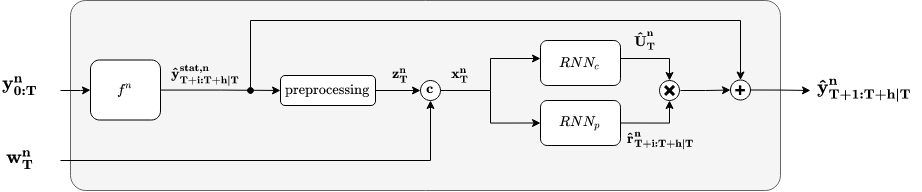
\includegraphics[width=1.2\linewidth]{figure/Regime_switching_recurrent_model}
  \caption{Hybrid model with weak signals architecture.}
\label{fig:architecture}
\end{figure}


\subsection{Hidden regime}

As $\hiddenregime$ is not observed, the loglikelihood of the observations cannot be written explicitly to train the model. Therefore we use Fisher's identity to compute the score function and write a gradient ascent algorithm to estimate simultaneously the weights of RNN-p and of RNN-c denoted by $\rnnparam = \{\rnnparam_c,\rnnparam_p\}$. The score is
\begin{equation}
\nabla_\theta \log p_\theta(\ts^n_{T+1:T+h}|\ts^n_{1:T}) = \mathbb{E}\left[\nabla_\theta \log p_\theta(\ts^n_{T+1:T+h},U_T^n|\ts^n_{1:T})\middle|\ts^n_{1:T+h}\right]\,,
\end{equation}
\\
where the joint likelihood $p_\theta(\ts^n_{T+1:T+h},U_T^n|\ts^n_{1:T}) = p_\theta(U_T^n|\ts^n_{1:T})p_\theta(\ts^n_{T+1:T+h}|U_T^n,\ts^n_{1:T})$ is given by \eqref{eq:full:model} and the expectation is under the posterior distribution of $U_T^n$ given $\ts^n_{1:T+h}$.
A complete description of the training process can be found in Appendix.



\section{Fashion dataset with external weak signals}
\label{sec:dataset}
%In image of language processing, there are available reference datasets covering varieties of applications. However, for time series forecasting, there is a lack of large, rich and public datasets where neural network approaches can express their potential. 
%\textcolor{red}{Other datasets for time series (see Alice paper on the SMC Transformer): air quality, weather, energy, Covid. These datasets exist but no easy weak signals to derive from them i guess. }
%M4 and M5 competitions\textcolor{red}{Add link in footnote} provide a large amount of time series data but they show several limitations. For example, the M4 dataset does not propose external signals in addition to the target time series. Conversely, the M5 dataset does include weak signals, but like other sales datasets \citep{C.Favorita}, it includes a majority of sporadic time series that cannot be included straightforwadly in a statistical model, see \citep{makridakis2020m5}. With this paper, we aim at overcoming this limitation of available datasets for time series forecasting with the first fashion dataset including external weak signals.

%With this paper, we provide the first dataset dedicated to fashion. Our fashion dataset is built with a high throughput computer vision systems analysing every day images shared on social networks. Aggregating detected clothes by trends, we create for the first time thousand of time series representing fashion trends life on social media. Moreover, our sequences show desirable properties. They have all the same length, weekly time step, shared behaviours, no sporadic sequence and no missing values. We provide publicly a selection of $\numberts$ anonymized fashion trends for men and women, on 9 differents categories and 5 geozones. An overview of it can be found in table 1.

\subsection{Fashion dataset}

With this paper, we provide the first dataset dedicated to fashion. Our fashion dataset is built with a high throughput computer vision systems analysing every day images shared on social networks. Aggregating detected clothes by trends, we create for the first time thousand of time series representing fashion trends life on social media. Our sequences have all 261 time steps, from 2015-01-05 to 2019-12-31 with weekly values and no missing walues. Each time series is normalized in order to remove social networks biases and their values lie between 0 and 1. The proposed fashion dataset contains $\numberts$ anonymized fashion trends for men and women, on 9 differents categories and 5 geozones. An overview of it can be found in table 1.

With in-house fashion experts, we selected especially a collection of $\numberts$ fashion trend in order to represent finely the issues that face the fashion industry. A large part of our time series are quite stable, their seasons and evolutions are regular. However, some sequences show interesting behaviours with sudden changes. We call them emerging or declining trends depending of the change direction. A central point of our work is to accurately detect and forecast these trends.

%With only the historical data, predict this breaking point is challenging and some time impossible. 

%a large part of this One central point is to accurately detect and forecast these trends. 

%Our sequences show several desirable properties: same length (from 2015-01-05 to 2020-09-01), same yearly seasonality, shared behaviours and no missing values. We provide publicly a selection of $\numberts$ anonymized fashion trends for men and women, on 9 differents categories and 5 geozones. An overview of it can be found in table 1.


%a rich dataset gathering 14000 time series of fashion trend occurance on social medias. we build our  Every day images shared on social networks are analyzed thanks to a high throughput computer vision systems. Aggregating detected clothes by trends, we create thousands of time series with the same good properties: : from 2015-01-05 to 2020-09-01. Each time series is normalized in order to remove social networks biases and their values lie between 0 and 1. The proposed fashion dataset contains $\numberts$ anonymized fashion trends for men and women, on 9 differents categories and 5 geozones. An overview of it can be found in table 1.

%Heuritech is the first company to adopt a data-intensive approach  for the fashion forecasting. 
%Every day images shared on social networks are analyzed thanks to a high throughput computer vision systems. Aggregating detected clothes by trends, we create thousands of time series with the same good properties: same weekly seasonality, shared behaviours and the same length: from 2015-01-05 to 2020-09-01 \textcolor{red}{Add a few details here or in the appendix}. Each time series is normalized in order to remove social networks biases and their values lie between 0 and 1. The proposed fashion dataset contains $\numberts$ anonymized fashion trends for men and women, on 9 differents categories and 5 geozones. An overview of it can be found in table 1.



\begin{table*}
  \caption{Fashion time series overview. For each couple geozone/category, we give the number of female and male trends (Female/Male)}
  \label{sample-table}
  \centering
  \resizebox{\textwidth}{!}{
  \begin{tabular}{lllllllllll}
    \hline
    &  Top  & Pants & Short & Skirt & Dress & Coat & Shoes & Color & Texture &  \\
    \hline
United States & 411/208 & 149/112 & 47/22 & 29/- & 20/- & 208/151 & 293/86 & 38/44 & 85/81\\
     Europe & 409/228 &  134/114 & 48/21 & 28/- & 20/- & 211/159 & 303/78 & 41/42 & 87/74\\
     Japan &  403/218 & 136/107 & 49/31 & 28/- &  23/- & 185/149 &  311/78 & 46/42 &  92/65\\
     China &  424/202 & 147/114 & 46/29 & 27/- &  27/- & 178/161 &  310/78 & 41/47 &  88/77\\
     Brazil &  431/222 & 134/117 & 49/27 & 30/- &  28/- & 203/152 & 311/76 & 48/41 & 107/84\\
     \hline
     Total & 2078/1078 & 700/564 & 239/130 & 142/- & 118/- & 985/772 & 1528/396 & 214/216 & 459/381 & \numberts\\
    \hline
  \end{tabular}
  }
\end{table*}

\subsection{Weak signal}

In addition to this large dataset we design for each sequence several weak signals.  Firstly, we create a specific fashion-oriented panel of micro-influencers. In theoretical fashion dynamics \citep{rogersdiffusion}, different categories of adopters follow a trend in succession, resulting in several adoption waves. With this specific panel, we aim at detecting the first waves announcing emerging trends or the collapse of other ones. By analyzing images shared by this specific panel on social medias, we create a first weak signal named \textit{fashion-forwards} for each of the previous trends. We also analyzed only a specific part of social media users depending of the number of followers. With three thresholds we created the following external signals : \textit{followers-low}, \textit{followers-mid} and \textit{followers-high}. Again, the motivation here is to detect behaviour gaps between these three segments that could announce bigger changes in the main signal.These extra signals are frequently sparse for micro trends and they often lack of interest for common fashion trends. However on several examples, they are fundamental to detect the future fashion evolution. 


%\subsection{Emerging/Declining fashion trend}


%One of the main objectifs of the fashion industry is to correctly understand and anticipate the futur tendances. 
%With in-house fashion experts, we selected a collection of $\tsnumber$ fashion trend representing finely the issues that face the fashion industry. Our dataset gather 3 types of trends, the common trends, the declining trends and the emerging trends. 


%A large part of our time series are regular, their evolutions are slow and constant in time.



%A large part of these trends are commom, their evolutions are regular and well anticipated. In addition to these trends, we find two   

%One of the today main objectifs of the fashion industry is to drastically reduce the massive waste due to wrong inventory decisions, see for instance \citep{}. With our new dataset, we want to create a focus at detecting precisely 


%The first one represents users with few followers, the second one is made of users with a moderate amount of followers and the last one gathers superstar and users of any fields with thousands of influencers. Again, the motivation here is to detect behaviour gaps between these three segments that could announce bigger changes in the main signal.


%At the end, we have for each trends 4 linked weak signals representing this trends on a specific panel of social media users. These extra signals are frequently sparse for micro trends and they often lack of interest for common fashion trends. However on several examples, they are fundamental to detect the future fashion evolution. 

\subsection{Example}

As an example, an impressive emerging fashion trend is represented in Figure 2, see other examples in Appendix~\ref{}. It shows the evolution of one shoes trends on social media and its linked \textit{fashion-forward} weak signal. During the first 3 years, common users and the panel of mode-influencers share the same behaviour. The trend start to boom in the mainstream people during the first month of 2018. However, we can detect early signals in the fashion-forward panel at the end of 2017. Early adopters started to change there behaviour and show more frequently the trend on social media. With fashion influence dynamics, the new tendency spreads to every part of social media users. Finally, after a pick reached at the end of 2018 for the fashion-influencers, a regular decrease appear. %They leave gradually the old trend to focus more on the latest or propose new ones. 

\begin{figure}
  \centering
    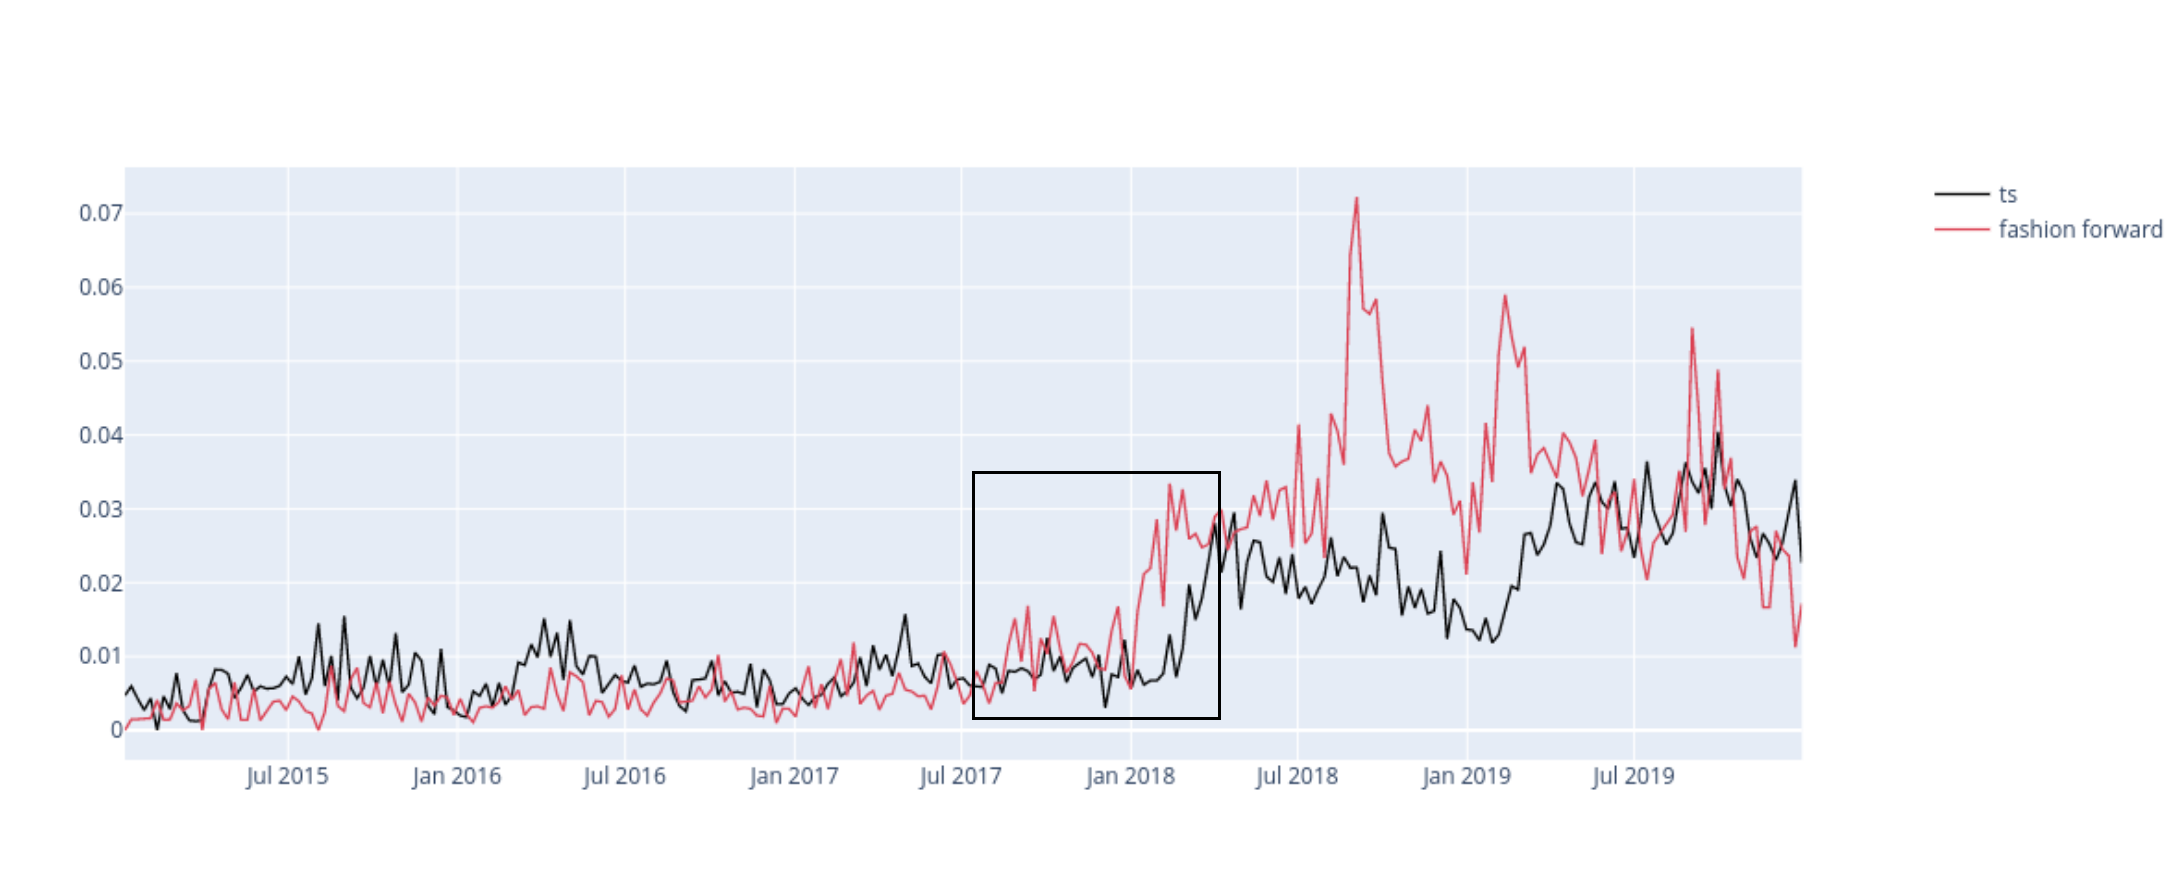
\includegraphics[width=1.\linewidth]{figure/emergering_trend.png}
  \caption{A shoes trend of our dataset. In black the main signal and in red its associated \textit{fashion-forward} weak signal. The Gap between our two signals in the end of 2017/beginning of 2018 announces the future explosion of the fashion trend. \textcolor{red}{Provide other examples in the appendix to hightlight the variety of the proposed data.}}
\end{figure}





\section{Experimental results}
\label{sec:exp}
%In this section, we evaluate how our hybrid framework is able to deal with the fashion dataset and leverage our complex external weak signals. To lead our experience, we keep hide the last year of each time series as our test set. For each method and each time series, based on the first five years of data, we predict the last year and compute our accuracy on it.

\subsection{Training}

To train our hybrid model, we split our dataset in 3 parts, train,eval and test set. We use the 3 first years as our train set, we keep the 4th year for our eval set and we hide the last year for our test set. We train our hyrid model to compute a one-year ahead prediction with $\window$ and $\lag$ equal to 52. In order to increase our train set, we use a moving window that provide 53 input/output couples per sequences, being 530000 couples in total. An example of our splitting is shown in  Figure~\ref{fig:train_eval_test_set}. All our code is developed in Python using the Tensorflow library. It allows the use of a GPU to speed up the trainig process.

For the first parametric per-time-series models, we used existing Python or R librarys to set the different parameters $\statparam^n$. There are then fixed during the training of the recurrent models.
For $\classifier$ and $\predictor$, we built an architecture summaryse in Figure~\ref{fig:rnnarchi}. There are both composed of 3 LSTM layer and a different final Dense layer to provide the correct output. After the $\classifier$ final dense layer, we add a sigmoid activation to return a probability. We use 2 Adam otpimizers with the same learning rate equal to ??? and we fix the batch size at 64. At the end, we use the eval set to fix the $\threshold$ parameter that determine, depending of the output of $\predictor$, when use the $\predictor$ correction. 

We propose two versions of our regime switching hybrid recurrent model. The first one is an hybrid model with an additive exponential smoothing model as the reference. For the second one, we use the TBATS approach as the reference.

\begin{figure}
  \centering
    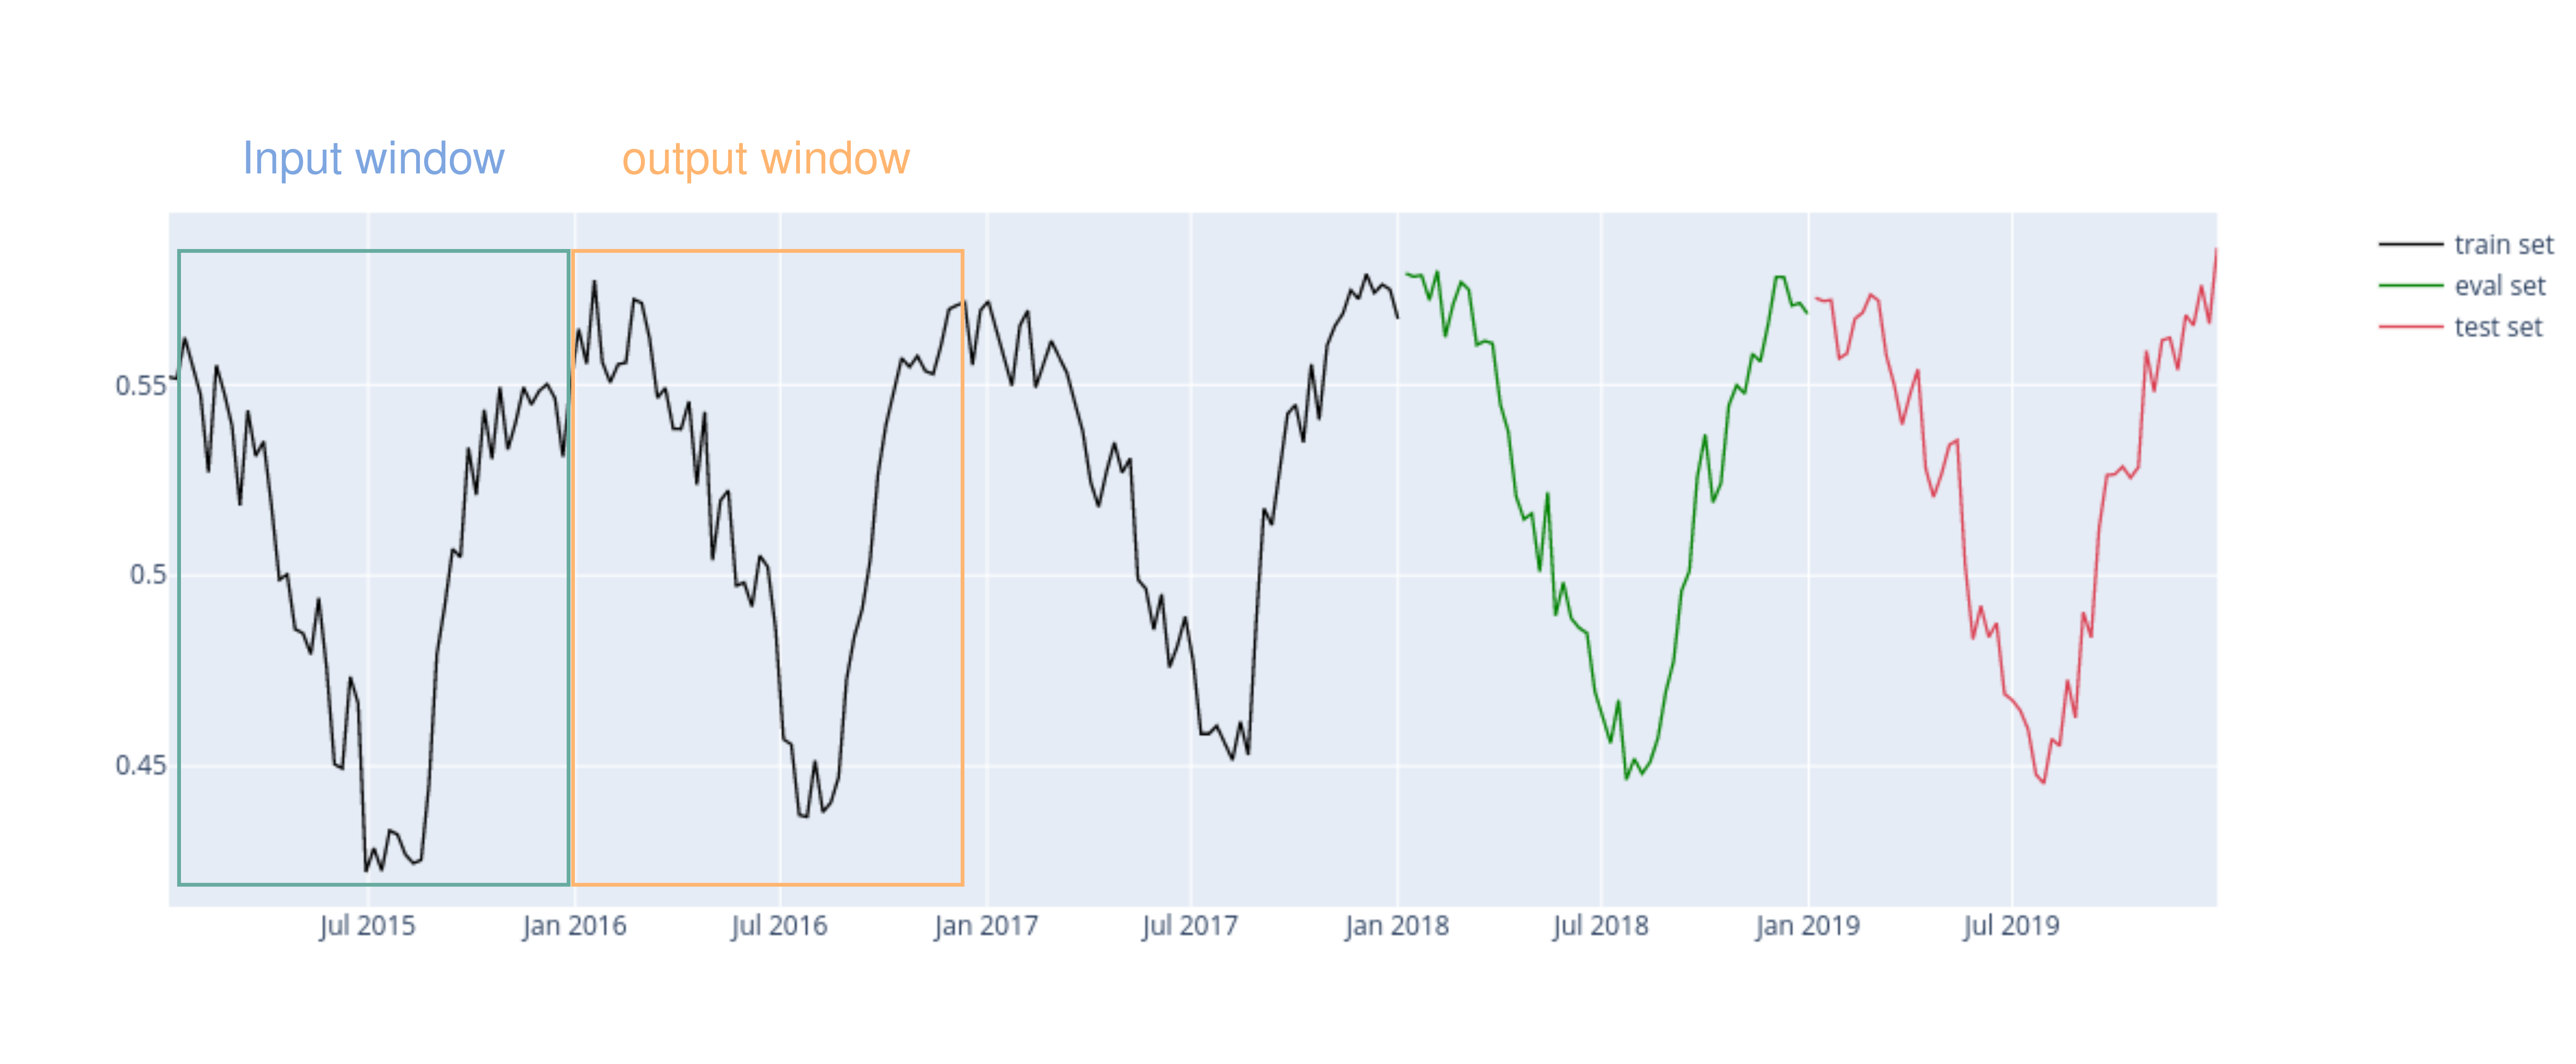
\includegraphics[width=1.\linewidth]{figure/train_eval_test_set}
  \caption{$\classifier$ and $\predictor$ architecture.}
\label{fig:train_eval_test_set}
\end{figure}

\begin{figure}
  \centering
    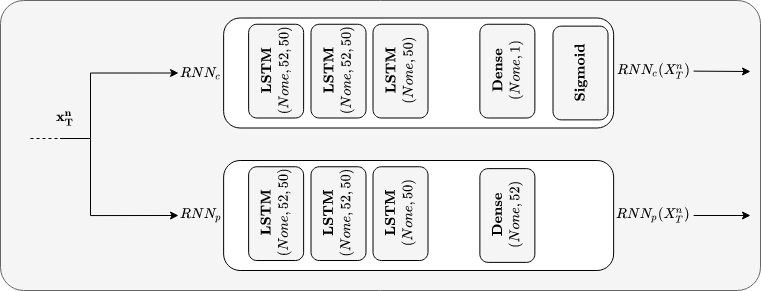
\includegraphics[width=0.8\linewidth]{figure/rnn_archi}
  \caption{$\classifier$ and $\predictor$ architecture.}
\label{fig:rnn_architecture}
\end{figure}


%To train our hybrid models, we made the choice of don't using the original code of the hybrid method provided during the M4 competition. Indeed, the proposed implementation is difficult to use in a more general framework and it is quite slow because it doesn't enable the use of GPU. Thereby, we propose with this paper, a new version of the hybrid framework, including the original multiplicative model and the new additive one. 
%Our code is developed in Python using the Tensorflow library and it allows the use of a GPU to speed up the training process contrary to other methods \textcolor{red}{\cite{} developed for the M4 competition}. In addition, our approach offers the possibility of providing forecasts for a totally  new collection of sequences without retraining the entire hybrid model. Given a new time series,  the weights of the error-corrector recurrent model are frozen and only the new time-series-specific statistical model has to be trained.% It remains the responsibility of the users to provide new sequences sharing same behaviours than the dataset using for the training to keep the same accuracy level.

%For more details about the general hybrid training, a complete description of the training process can be found in the M4 hybrid model paper or in an interesting application of the method on electric load forecasting, see \citep{dudek2020hybrid}.

%\textcolor{red}{Detail here or in the appendix the training details: number of samples, optimizers, learning rates, etc.}

%\vspace{.2cm}

%\textcolor{red}{Detail Train/test split.}

\subsection{Benchmarks, hybrid models and Metrics}

As benchmarks, we chose several well-known statistical methods and deep learning approaches. Using the R package \texttt{forecast} and the Python packages \texttt{statsmodels, tbats} , we compute for each time series a prediction with the following methods: \textit{snaive}, \textit{ets}, \textit{stlm}, \textit{thetam}, \textit{tbats} and \textit{auto.arima}. \textit{snaive} forecasts are only the repetition of the last same past period. \textit{ets} model is an additive exponential smoothing with a level component and a seasonal component. \textit{stlm} approach use a multiplicative decomposition and models the seasonality adjusted time series with an exponenantial smoothing model. \textit{Thetam} model decompose the original signal in $\theta$-lines, forecast each one separately and recompose them to produce the final forecast. \textit{tbats} is a powerful statistical model using a trigonometrical seasonality modelization. The last one \textit{auto.arima} is the R implementation of ARIMA model with an automatic selection of the best parameters. A complete description and references for these models can be found in \citep{packageforecast}. As a deep learning approach, we considered a full LSTM (\textit{lstm}) neural network composed of 3 LSTM layers of shape 50 and a final Dense layer of shape 52.

Against these models, we propose our two versions of our regime switching hybrid reccurent model (rshm) called respectively rshm-ets and rshm-tbats according to the per-time-series model choice.
%Against these models, we propose two versions of our regime switching hybrid recurrent model \textit{rshm}. The first one, that we name \textit{rshm-ets}, is the hybrid model with an additive exponential smoothing model as parametric model. For the second one, we use the TBATS approach as paramteric model and we named it \textit{rshm-tbats}. 
%To reach a higher accuracy level we also propose an ensembling (\textit{ensembling} of our hybrid approach using the FFORMA method created during the M4 competition, see \citep{fforma}). 
For our two versions, in a first time, we propose a version without our weak signal called \textit{rshm-ets} and \textit{rshm-tbats}. Then we evaluate our hybrid framework with the inclusion of our weak signals (ws) referred to as \textit{rshm-ets-ws} and \textit{rshm-tbats-ws}. In order to provide a fair comparison, we also train a \textit{lstm} with the weak signals named \textit{lstm-ws}.


To compare the different methods, we use the same metrics as in the M4 competition: the Mean Absolute Scaled Error (MASE), the Symmetric Mean Absolute Percentage Error (sMAPE) and the final M4 competition metric, the Overall Weighted Average (OWA) of the sMAPE and the MASE defined as follows:
\begin{align*}
\mathrm{MASE} &= \frac{T-m}{h}\frac{\sum_{i=1}^h |Y_i - \hat{Y}_i| }{\sum_{i=1}^{T-m} |Y_i - Y_{i-m}|}\,,\\
\mathrm{sMAPE} &= \frac{1}{h} \sum_{i=1}^h \frac{2|Y_i - \hat{Y}_i|}{|Y_i| + |\hat{Y}_i|}\,,\\
\mathrm{OWA} &= \frac{1}{2}\left(MASE/MASE_{snaive} + sMAPE/sMAPE_{snaive}\right)\,,
\end{align*}

where $\hat{Y}$ is a model prediction, $\lag$ is the horizon, $m$ the seasonality and $MASE_{snaive}$ is the $MASE$ computed with the $snaive$ model prediction, idem for the $sMAPE_{snaive}$.



Detecting emerging and declining trends is a crucial issue for the fashion industry. A correct or incorrect prediction could lead to good returns or massive waste due to overstock or unsold clothes. In a given year, we define an increasing trend as a trend that do more than 10\% of growth in term of Year and Year.In the same way, we define a decreasing trend as a trend that decline of 10\% or more. We classify other trends as flat trends. On the test set, the year 2019, we have 1871 increasing trends, 2016 decreasing trends and 6113 flat trends. In addition to the accuracy metrics, we compare also the different methods on this classification task.



%As detecting emerging and declining trends is a fondamental issue that is facing the fashion industry, we evaluate also the different methods on this task. In a given year, we define an increasing trend as a trend that do more than 10\% of growth in term of Year and Year.A decreasing trend is a trend that decline of -10\% or more. We classify the other trend as flat trend. On the test set, the year 2019, we have 1871 increasing trends, 2016 decreasing trends and 6113 flat trends. We evaluate all the methods on this classification task.



%\textcolor{red}{where $\mathrm{smape_{snaive}}$ and $\mathrm{mase_{snaive}}$ are}.

%\subsection{Results for XXX Dataset}
%\textcolor{red}{If possible, a few results of the hybrid approach without weak signals on a dataset other than Heuritech.}






\subsection{Result for Heuritech Fashion dataset}

%\textcolor{red}{Add a figure of a time series with all models (and others in Appendix).}

%\vspace{.2cm}

%\textcolor{red}{Add a table with the results on the trends classifications used in Heuritech.}

The Table ??? present the final result for all our methods on the three metrics presented above.
\begin{itemize}
	\item For the statistical models, we can see a large domination of the TBATS model with a MASE equal to ... It is one of the main reason why we use this model on one of our hybrid framwork as the parametric model. However, we can see that the full LSTM model \textit{lstm} is the best model over our benchmarck candidates. This result show that, with a large dataset, deep learning model can outperform the traditional approaches on average. An example of prediction of all the benchmarck methods is displayed in the Figure ????.
	\item Our two different regime switching hybrid model achieve higher level of accuracy compare to the \textit{ets} or \textit{tbats} results. For the \textit{rshm-ets}, we pass from ??? for the \textit{ets} model alone to ???? for the hybrid model. Its $\classifier$ threshold $\threshold$ was fix at ???. With this threshold, the error-corrector model correct ???? sequences of the $\numberts$. On these corrected time series, compare to the \textit{ets} apporach, our appoach MASE fall from ??? to ???. However \textit{rshm-ets} doesn't succed at outperform some of the benchmarck model, for example \textit{tbats} of \textit{lstm}. The \textit{rshm-tbats} version clearly outperform all the previous model. Based on a \textit{tbats} model, wich already achieve a interesting level of accuracy, \textit{rshm-tbats} reach the higher level of accuracy with a MASE equal to ????, that is -??? compare at the top-2 model. With a threshold fixed at ???, this version of our hybrid framework correct ??? sequences of the $\numberts$. An example of our two regime-switching hybrid recurrent model is presented in the Figure ....
\end{itemize}

\begin{table*}
  \caption{Results summary (Mean/Median) on our Fashion dataset. In a first time, we train our hybrid approaches without our external weak signals.}
  \label{sample-table}
  \centering
  \begin{tabular}{lllllll}
    \hline
    &  MASE  & MASE-std & SMAPE & SMAPE-std & OWA & OWA-std  \\
    \hline
     \textit{snaive} & 0.983/0.936 & 0.33 & 27.68/24.42 & 15.0 & 1./1. & 0.\\
     \textit{ets} & 0.983/0.936 & 0.33 & 27.68/24.42 & 15.0 & 1./1. & 0.\\
     \textit{thetam} & 0.983/0.936 & 0.33 & 27.68/24.42 & 15.0 & 1./1. & 0.\\
     \textit{stlm} & 0.983/0.936 & 0.33 & 27.68/24.42 & 15.0 & 1./1. & 0.\\
     \textit{tbats} & 0.983/0.936 & 0.33 & 27.68/24.42 & 15.0 & 1./1. & 0.\\
     \textit{auto.arima} & 0.983/0.936 & 0.33 & 27.68/24.42 & 15.0 & 1./1. & 0.\\
     \textit{lstm} & 0.983/0.936 & 0.33 & 27.68/24.42 & 15.0 & 1./1. & 0.\\
     \textit{rshm-ets} & 0.983/0.936 & 0.33 & 27.68/24.42 & 15.0 & 1./1. & 0.\\
     \textit{\textbf{rshm-tbat}} & 0.983/0.936 & 0.33 & 27.68/24.42 & 15.0 & 1./1. & 0.\\
    \hline
  \end{tabular}
\end{table*}




%In a first place, Table 2 shows the final accuracy of the statistical models, the LSTM model and our 2 hybrid models without external data. Even without the weak signals, our 2 hybrid approaches largely outperform the statistical references. The multiplicative model show the best accuracy with a OWA equal to 0.875. We can note that the additive model slightly under-performs the traditional multiplicative one on average. This doesn't show a weakness of the additive version but more that a large part of our dataset is more-suited for multiplicative modelization. At the end, the strength of training both methods, additive and multiplicative, is in the final porposed ensembling \textit{ensembling} that combines the two approaches with the FForma ensembling.

%In a second place, Table 3 shows the evaluation of our 4 trained hybrid models: the 2 previous ones without weak signals, and our 2 full hybrid models with weak signals. We present also the accuracy of a simple LSTM model with and without weak signals. We can show the impressive improvement due to our external signals. Again, the multiplicative method achieves the best accuracy with OWA metric equal to 0.860. We propose like previously, an ensembling mixing our two full hybrid models with weak signals and it reach the high level of accuracy with an OWA equal to 0.849.

%In a third place, table 4 presents the result of our inference process. We split our dataset in five equal parts of 2800 sequences and hide the last year for each trends. Then, like a cross validation, we train a model on 4 parts and compute its accuracy on the last one on the last year. The model never saw the last part so we use our inference process to compute predictions. With a permutation of the parts, we can repeat the process and train 5 models, each trained on a specific pool of 4 parts and tested on the remaining part of the dataset. For each hybrid model (additive/multiplicative with and without weak signals) Table 4 shows the average accuracy and the Standard Deviation of the 5 trained hybrid models. We can see that our inference process achieve really accurate results and practically the same that our hybrid models trained on the entire dataset. These results prove that, even without having seen a sequence during the training, if the time series share same behaviours that the training sample, our hybrid approaches can perfectly compute accurate predictions. Furthermore, the Standard Deviation is really low for all our metrics. This result shows that our hybrid framework is robust and reach constant accuracy level on large dataset.


With our results, we can make two interesting conclusions. Firstly, the regime switching hybrid framework is a really promising framework. By mixing the performance of local parametric models and a global DNN, our two versions clearly outperform traditional statistical methods. Furthermore, this framework is totally suited for dealing with external signals. With a fine pre-processing and a well-designed architecture, our two models succeed at leveraging our complex extra data and reach an impressive accuracy levels. Secondly, our results bring to light the quality of our new Fashion dataset. We saw that the full LSTM model \textit{lstm} outperforms all time series specific models. This show that our dataset is well suited to train complex neural network architectures able to learn information cross sequences. With the addition of our weak signals, we give a totally new dimension to our fashion dataset. Our results show that our external weak signals hide a complex but usable predictive power by DNN architecture. By making it publicly available, we hope that it will enhance the set of datasets for time series forecasting. 


\subsection{Discussion}


%\begin{table*}
 % \caption{Comparison between our hybrid models without and with our external weak signals, (Mean/Median)}
  %\label{sample-table}
  %\centering
  %\begin{tabular}{lllllll}
   % \hline
    %&  MASE  & MASE-std & SMAPE & SMAPE-std & OWA & OWA-std \\
    %\hline
    %lstm & 0.881/0.824 & 0.34 & 24.41/21.56 & 12.81 & 0.895/0.885 & 0.11 \\
    %lstm-ws & 0.869/0.814 & 0.33 & 24.56/21.33 & 14.40 & 0.890/0.874 & 0.132 \\
    % hybrid-add & 0.863/0.812  & 0.32 & 24.17/21.36 & 13.0 & 0.877/0.880 & 0.08 \\
     %hybrid-mul & 0.858/0.817 & 0.30 & 24.06/21.30 & 13.0 & 0.876/0.873 & 0.11 \\
  %   hybrid-add-ws & 0.852/0.807 & 0.30 & 24.03/21.17 & 13.0 & 0.872/0.869 & 0.10 \\
%     hybrid-mul-ws & 0.836/0.798 & 0.29 & 23.67/20.87 & 12.9 & 0.860/0.858 & 0.12 \\
 %    Ensembling & 0.827/0.787 & 0.29 & 23.43/20.63 & 12.8 & 0.849/0.849 & 0.11\\
  %  \hline
  %\end{tabular}
%\end{table*}



%\begin{table*}
 % \caption{Cross-Validation. we split our dataset in 5 equal parts. We train for each hybrid approach, 5 models on 4 specific parts of the dataset and we test them of the remaining parts with our inference process.}
  %\label{sample-table}
  %\centering
 % \begin{tabular}{lllllll}
  %  \hline
   % &  MASE  & MASE-std & SMAPE & SMAPE-std & OWA & OWA-std \\
   % \hline
   %  hybrid-add & 0.861  & 0.004 & 24.16 & 0.18 & 0.877 & 0.002 \\
   %  hybrid-mul & 0.856 & 0.008 & 23.95 & 0.25 & 0.870 & 0.005 \\
   %  hybrid-add-ws & 0.848 & 0.004 & 24.00 & 0.18 & 0.869 & 0.002 \\
   %  hybrid-mul-ws & 0.844 & 0.010 & 23.74 & .20 & 0.863 & 0.006 \\
   % \hline
  %\end{tabular}
%\end{table*}




\section{Conclusion}
\label{sec:discussion}
In this paper, we propose the first hybrid model including external weak signals for time series forecasting. We show that hybrid framework is a really promising way. With its extended error-corrector DNN part, it is clearly well-suited for dealing with any kind of external signals in order to correct weaknesses of first parametric models. Furthermore, With our additive version, we show that the hybrid model is not frozen in it original form. Thereby, future research explorations would be to improve its framework with new per-time-series approaches and test new error-corrector DNN part like the recent Transformer model.

With this first contribution, we join the first fashion dataset gathering \numberts\ mode times series and a complex collection of extra signals. We believe that this dataset hide really fine dynamics and interactions where complex models would express their potential. By making it publicly available, we hope that it will enhance the set of datasets for time series forecasting and pave the way for further explorations.


\bibliography{iclr2022_conference}
\bibliographystyle{iclr2022_conference}

\appendix

\section{Fashion Dataset overview}



\section{Hidden regime algorithm}

In our framework, we assume that our sequence are generated with a regime with 2 hidden regime. As this regime, noted $\hiddenregime$, is never observed, we can compute explicitely the following quantity : 
%$p(\ts^n_{T+1:T+h}|\ts^n_{1:T})$


%Based on the Expectation-Maximization (EM) algorithm and the Fisher's identity, we write a new algorithm to estimate jointly $\theta = \{\theta_p,\theta_c\}$, the weights of RNN-p and of RNN-c. 

%During our training, we note $\theta^{(t)}$ the value of $\theta$ at an epoch $t$.


%\begin{equation}
%\nabla_\theta \log p_\theta(\ts^n_{T+1:T+h}|\ts^n_{1:T}) = \mathbb{E}\left[\nabla_\theta \log p_\theta(\ts^n_{T+1:T+h},U_T^n|\ts^n_{1:T})\middle|\ts^n_{1:T+h}\right]\,,
%\end{equation}




\section{}




\textcolor{red}{details to add in appendix.} \textcolor{red}{Assume that $\theta_p$ is the current value for the weights of the RNN-p and the RNN-c and write $\omega_p^n = \mathbb{P}_{\theta_p}(U_T^n = 1|\ts^n_{1:T+h})$. Note that
$$
\omega_p^n \propto \mathbb{P}_{\theta_p}(U_T^n = 1|\ts^n_{1:T})p_{\theta_p}(\ts^n_{T+1:T+h}|U_T^n=1,\ts^n_{1:T})\,.
$$
Then,
\begin{multline*}
\nabla_\theta \log p_\theta(\ts^n_{T+1:T+h}|\ts^n_{1:T}) = \omega_p^n\nabla_\theta \log p_\theta(\ts^n_{T+1:T+h},U_T^n=1|\ts^n_{1:T})\\
+ (1-\omega_p^n)\nabla_\theta \log p_\theta(\ts^n_{T+1:T+h},U_T^n=0|\ts^n_{1:T})\,.
\end{multline*}
The loss function is then given by
\begin{multline*}
\theta\mapsto - \omega_p^n \log p_\theta(\ts^n_{T+1:T+h},U_T^n=1|\ts^n_{1:T})\\
- (1-\omega_p^n) \log p_\theta(\ts^n_{T+1:T+h},U_T^n=0|\ts^n_{1:T})\,,
\end{multline*} 
where no gradient is computed on $\omega_p^n$. In both terms, $\log p_\theta(U_T^n=0|\ts^n_{1:T})$ and $\log p_\theta(U_T^n=0|\ts^n_{1:T})$ are simply given by the output of the FFNN.  Choices for the model.
\begin{itemize}
\item In the case where the  $\varepsilon^n_{T+i}$ are Gaussian and independent, up to an additive constant
$$
\log p_\theta(\ts^n_{T+1:T+h}|U_T^n=0,\ts^n_{1:T}) = -c\sum_{i=1}^{h}(\ts^n_{T+i}  - \tspred^{stat,n}_{T-w+i|T-w})^2
$$
and
\begin{multline*}
\log p_\theta(\ts^n_{T+1:T+h}|U_T^n=1,\ts^n_{1:T})\\
 = -c\sum_{i=1}^{h}(\ts^n_{T+i}  - \tspred^{stat,n}_{T-w+i|T-w} - \meants^n_T\times \rnnmodel(\fullconcatinput^n_T)_{T+i})^2\,.
\end{multline*}
Choice of $c$ ?
\item In the case where the  $\varepsilon^n_{T+i}$ are Laplace and independent, up to an additive constant
$$
\log p_\theta(\ts^n_{T+1:T+h}|U_T^n=0,\ts^n_{1:T}) = -c\sum_{i=1}^{h}|\ts^n_{T+i}  - \tspred^{stat,n}_{T-w+i|T-w}|
$$
and
\begin{multline*}
\log p_\theta(\ts^n_{T+1:T+h}|U_T^n=1,\ts^n_{1:T})\\
 = -c\sum_{i=1}^{h}|\ts^n_{T+i}  - \tspred^{stat,n}_{T-w+i|T-w} - \meants^n_T\times \rnnmodel(\fullconcatinput^n_T)_{T+i}|\,.
\end{multline*}
Choice of $c$ ?
\end{itemize}}

\end{document}
